%\subsection{The UK Biobank cohort}
The UK Biobank is a large-scale prospective cohort study comprising approximately 500,000 participants aged 40-69 years at recruitment between 2006 and 2010 across the United Kingdom~\citet{Sudlow2015UKBiobank}. This population-based resource represents one of the most comprehensive biomedical databases worldwide, systematically integrating demographic information, lifestyle questionnaires, physical measurements, biological samples, multi-omics data, and longitudinal electronic health record (EHR) linkage. The core of our analytical framework resides in the definition of a high-dimensional phenotyping space, designed to capture the longitudinal evolution of cardiometabolic conditions. We defined 24 primary cardiometabolic diseases as the core focus of the comorbidity network, alongside 76 risk factors selected based on established epidemiological literature. Phenotype definitions were developed through expert clinical consultation to ensure consistency with diagnostic criteria and epidemiological standards. We adopted a multi-source ascertainment strategy that integrates three distinct clinical domains: ICD-10 diagnosis codes and OPCS-4 procedure codes indicating surgical or interventional treatment (1) from hospital inpatient records; (2) from primary care data; and (3) laboratory measurements from primary care data. This multi-source definition strategy enhances phenotype sensitivity by capturing patients' history through diverse clinical touchpoints. The 24 primary diseases encompass major cardiovascular conditions (acute myocardial infarction, coronary disease, heart failure, atrial fibrillation, ventricular arrhythmias, cardiac arrest, cardiomyopathies), valvular heart diseases (aortic, mitral, and tricuspid valve disorders), vascular diseases (cerebrovascular disease, hemorrhagic stroke, aneurysm and dissection, peripheral vascular diseases, acute pulmonary embolism), advanced cardiovascular interventions (pacemaker implantation for conduction delay, heart transplantation for end-stage heart failure), metabolic conditions (diabetes mellitus, dyslipidemias), hypertension, and progressive stages of renal dysfunction (acute kidney injury, chronic kidney disease stages 3-5, end-stage renal disease). In addition to the primary diseases, 76 risk factors were considered to adjust for confounding, including demographic and socioeconomic factors, family history of cardiovascular disease, lifestyle and anthropometric factors, clinical biomarkers, and comorbidities. Complete definitions and life-course incidences for each disease are provided in Supplementary Table~\ref{ST:table1} for the primary diseases and Supplementary Table~\ref{ST:table2} for risk factors. Longitudinal incidence distribution plots for each primary disease are shown in Supplementary Figure~\ref{supp_mat:SF0}. All phenotypes were mapped to the Medical Subject Headings (MeSH) vocabulary to enable integration with BioWordVec pretrained embeddings. After MeSH mapping, the final vocabulary comprised 24 unique main diseases and 76 unique risk factors (98 unique events). Information about the MeSH mapping is provided in Supplementary Tables~\ref{ST:table1} and~\ref{ST:table2}. We recorded 544,716 primary disease events and 3,285,210 risk factor events, with Figure~\ref{fig:main_dist_time_events_SF3} showing the temporal distribution of the disease events. Starting from 502,297 UK Biobank participants, we excluded individuals with fewer than three recorded main disease events during the life course. The final cohort comprised 113,973 participants. For each participant, we constructed longitudinal event sequences capturing temporal progression throughout their clinical history; details are provided in Section~\ref{subsection:seq_con}. %Phenotype terms were mapped to Medical Subject Headings (MeSH) vocabulary to enable integration with BioWordVec pretrained embeddings. %During MeSH mapping, Endstage Heart Failure and Heart Failure were consolidated into a single term. 

\begin{figure}
    \centering
    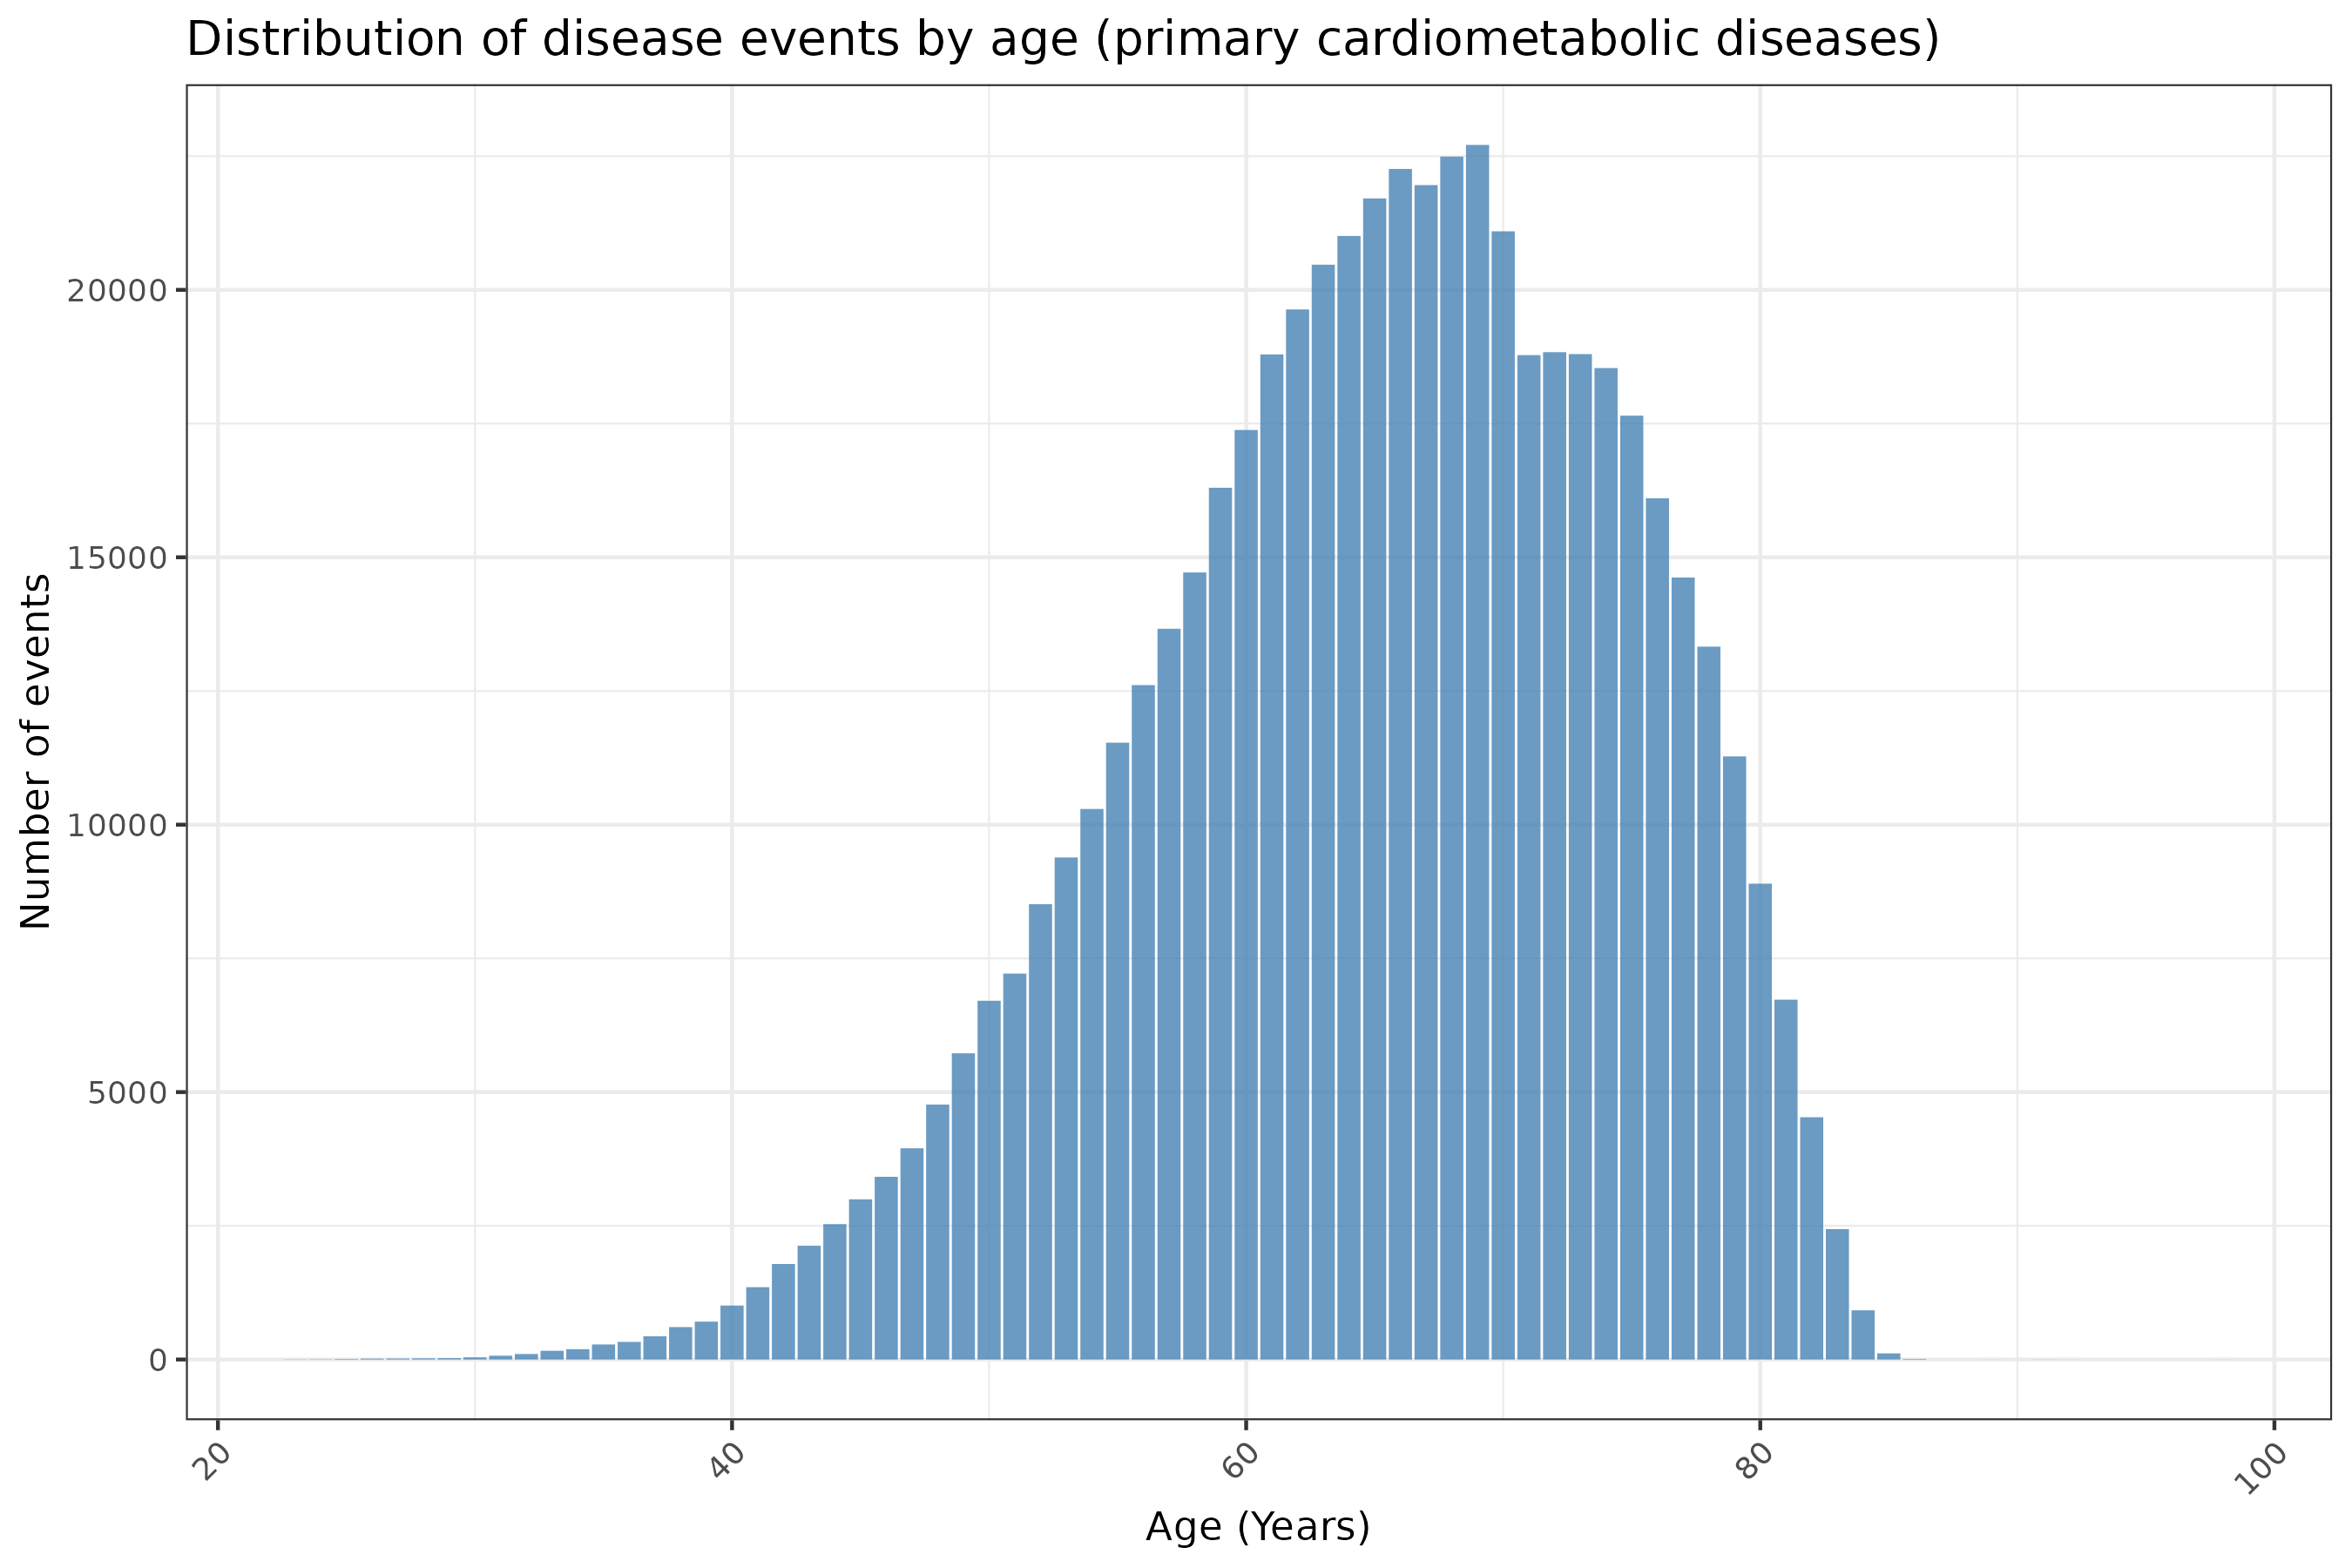
\includegraphics[width=\linewidth]{Figures/total_events_by_age.png}
        \caption{Distribution of event times for 24 primary cardiometabolic diseases.}
        \label{fig:main_dist_time_events_SF3}
\end{figure}

